%%%%%%%%%%%%%%%%%%%%%%%%%%%%%%%%%%%%%%%%%
% Short Sectioned Assignment
% LaTeX Template
% Version 1.0 (5/5/12)
%
% This template has been downloaded from:
% http://www.LaTeXTemplates.com
%
% Original author:
% Frits Wenneker (http://www.howtotex.com)
%
% License:
% CC BY-NC-SA 3.0 (http://creativecommons.org/licenses/by-nc-sa/3.0/)
%
%%%%%%%%%%%%%%%%%%%%%%%%%%%%%%%%%%%%%%%%%

%----------------------------------------------------------------------------------------
%	PACKAGES AND OTHER DOCUMENT CONFIGURATIONS
%----------------------------------------------------------------------------------------

\documentclass[paper=a4, fontsize=11pt]{scrartcl} % A4 paper and 11pt font size

\usepackage[T1]{fontenc} % Use 8-bit encoding that has 256 glyphs
\usepackage{fourier} % Use the Adobe Utopia font for the document - comment this line to return to the LaTeX default
\usepackage[spanish]{babel} % English language/hyphenation
\selectlanguage{spanish}
\usepackage[utf8]{inputenc}
\usepackage{amsmath,amsfonts,amsthm} % Math packages
\usepackage{graphicx}

\usepackage{sectsty} % Allows customizing section commands
\allsectionsfont{\centering \normalfont\scshape} % Make all sections centered, the default font and small caps

\usepackage{fancyhdr} % Custom headers and footers
\pagestyle{fancyplain} % Makes all pages in the document conform to the custom headers and footers
\date{}
\fancyhead{} % No page header - if you want one, create it in the same way as the footers below
\fancyfoot[L]{} % Empty left footer
\fancyfoot[C]{} % Empty center footer
\fancyfoot[R]{\thepage} % Page numbering for right footer
\renewcommand{\headrulewidth}{0pt} % Remove header underlines
\renewcommand{\footrulewidth}{0pt} % Remove footer underlines
\setlength{\headheight}{-1.6pt} % Customize the height of the header
\oddsidemargin=-0.5cm
\textwidth=17cm
\textheight=24cm


\numberwithin{equation}{section} % Number equations within sections (i.e. 1.1, 1.2, 2.1, 2.2 instead of 1, 2, 3, 4)
\numberwithin{figure}{section} % Number figures within sections (i.e. 1.1, 1.2, 2.1, 2.2 instead of 1, 2, 3, 4)
\numberwithin{table}{section} % Number tables within sections (i.e. 1.1, 1.2, 2.1, 2.2 instead of 1, 2, 3, 4)

\setlength\parindent{0pt} % Removes all indentation from paragraphs - comment this line for an assignment with lots of text

%----------------------------------------------------------------------------------------
%	TITLE SECTION
%----------------------------------------------------------------------------------------

\newcommand{\horrule}[1]{\rule{\linewidth}{#1}} % Create horizontal rule command with 1 argument of height

\title{	
\normalfont \normalsize 
\textsc{UNIVERSIDAD DE CANTABRIA, DEPARTAMENTO DE FÍSICA MODERNA} \\ [20pt] % Your university, school and/or department name(s)
\horrule{0.5pt} \\[0.4cm] % Thin top horizontal rule
\huge Física de Partículas Elementales (G71) \\ % The assignment title
\normalsize 4 Curso - Grado de Física - Doble Grado Física Matemáticas - Segundo Bloque - Final
\horrule{2pt} \\[0.5cm] % Thick bottom horizontal rule
}

\begin{document}

\maketitle % Print the title

\vspace{-2.5cm}

%----------------------------------------------------------------------------------------
%	PROBLEM 1
%----------------------------------------------------------------------------------------
\textbf{Cuestión 1.} Un haz de electrones y otro de positrones ambos no polarizados colisionan en el sistema centro de masas con una energía $\sqrt{s}=$ 5 GeV dando lugar a 
pares de muon-antimuon. ¿Cuál sería el momento de los muones resultantes?. \textbf{(0.25 puntos)}. Con la información dada, ¿sería posible estimar la proyección 
del momento del muon en la dirección inicial de los electrones?. Razona tu respuesta. \textbf{(0.25 puntos)}. En las condiciones dadas, ¿cuál sería el cociente
entre el número de muones detectados en la dirección inicial de los electrones ($\theta=0$) y en la dirección $\theta=\pi$. \textbf{(0.5 puntos)}. Supongamos ahora
que los electrones incidentes han pasado por un polarizador que sólo deja pasar electrones Left-Handed y que los muones resultantes se hacen pasar por un polarizador
que sólo deja pasar muones Right-Handed. ¿Cuál sería en este caso el cociente entre el número de muones detectados en $\theta=0$ y $\theta=\pi$?. \textbf{(0.5 puntos)}.
¿Cambiaría este último cociente si el experimento se realizase a $\sqrt{s}=90 GeV$? Razona tu respuesta. \textbf{(0.5 puntos)}. $m(\mu)=106$ MeV.
\\
\\
%----------------------------------------------------------------------------------------
%       PROBLEM 2
%----------------------------------------------------------------------------------------
\textbf{Cuestión 2.} Describe el concepto de quiralidad. \textbf{(0.5 Puntos)}. Explica razonadamente la relación que existe entre el concepto de quiralidad y 
la violación de Paridad que aparece en la fuerza débil. \textbf{(0.5 Puntos)}. Demuestra, usando únicamente la relación ${\gamma^\mu, \gamma^\nu}=2g^{\mu\nu}$, que
${\gamma^5, \gamma^\mu} = 0$. \textbf{(0.5 puntos)}. Deriva la forma de un espinor de partícula, autoestado del operador quiralidad con quiralidad Left-Handed. Razona
tu respuesta. \textbf{(0.5 puntos)}.  
\\
\\
%----------------------------------------------------------------------------------------
%       PROBLEM 3
%----------------------------------------------------------------------------------------
\textbf{Cuestión 3.} Madame Wu diseñó un experimento en el que un núcleo de cobalto decae en un núcleo de níquel, un electrón y un antineutrino: $Co\rightarrow Ni + e^{-} + \bar{\nu_e}$
en presencia de un campo magnético. El diagrama \ref{dibujo} muestra un esquema de este proceso para dos situaciones en las que el campo magnético está alineado
(derecha) o antialineado (izquierda) con el eje Z. En ambos casos el spin del cobalto y del níquel se alinea siguiendo el campo magnético. Puesto que el níquel tiene
una unidad menos de spin que el cobalto, el electrón y el anti-neutrino tendrán que compensar la pérdida de spin tal y como se indica en el diagrama. Asigna y calcula
los espinores de Dirac autoestados de la helicidad \ref{espinores} a cada uno de los electrones y anti-neutrinos en el diagrama, en función del momento $p$ y las masas
(asume $\phi=0$). \textbf{(0.5 Puntos)}. Asumiendo que la masa del neutrino es exactamente 0, uno de los diagramas tiene una probabilidad de ocurrir igual a 0. Indica
cuál y explica por qué en relación al elemento de matriz asociado a la fuerza débil mediada por un bosón W. \textbf{(0.5 Puntos)}. Usando los espinores de Dirac y los
operadores de proyección quiral demuestra lo mismo matemáticamente. \textbf{(1 Punto)}.
\\
\\
%----------------------------------------------------------------------------------------
%       PROBLEM 4
%----------------------------------------------------------------------------------------
\textbf{Cuestión 4.} ¿Qué es el isospin débil? \textbf{(0.5 puntos)}. ¿Cómo se relaciona el isospin débil con el hecho de que la fuerza débil tenga 3 bosones propagadores 
de fuerza? \textbf{(0.5 puntos)}. La fuerza débil viola la paridad porque sus cuadricorrientes son proporcionales a $g_V \gamma^\mu + g_A \gamma^\mu\gamma^5$ con $g_V$ y
$g_A$ constantes. ¿Por qué decimos que la violación de paridad obtenida cuando $g_V=1$ y $g_A=-1$ es máxima?. Pista: La cantidad de violación de paridad vieneda dada por
$\frac{g_Ag_V}{(g_A^2+g_V^2)}$?.\textbf{(0.5 Puntos)}. ¿Qué diferencia hay entre el boson gauge $W^3$ y el bosón Z?. \textbf{(0.5 puntos)}.
%----------------------------------------------------------------------------------------
\\
\\
%----------------------------------------------------------------------------------------
%       PROBLEM 5
%----------------------------------------------------------------------------------------
\textbf{Cuestión 5.} ¿Qué entendemos por el proceso de hadronización de un quark?. \textbf{(0.5 puntos)}. ¿Cómo explica la teoría de la fuerza fuerte el hecho de que
no se hayan observado mesones formados por dos quarks? (No hace falta demostrarlo matemáticamente). \textbf{(0.5 puntos)}. Un quark y un antiquark se aniquilan dando
lugar a otro quark y antiquark en un proceso mediado por la fuerza fuerte. Dibuja el diagrama de Feynman asociado indicando los nombres y cargas de las partículas
asociadas. \textbf{(0.5 puntos)}. Suponiendo que los quarks entrantes y salientes tienen color i, k y j, l respectivamente: ¿Qué forma tendría la expresión del 
matrix element? Explica las diferencias con respecto al mismo proceso pero mediado por la fuerza electromagnética. \textbf{(0.5 puntos)}. 
\\
\\


\begin{figure}[!h]
\begin{center}
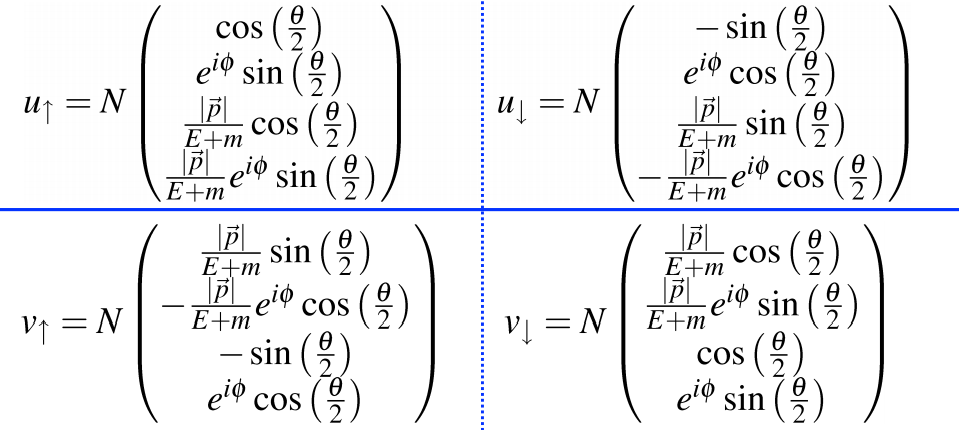
\includegraphics[width=0.6\linewidth]{espinores.png}
\end{center}
\caption{Espinores solución a la ecuación de Dirac y autoestados del operador helicidad.}
\label{espinores}
\end{figure}

\begin{figure}[!h]
\begin{center}
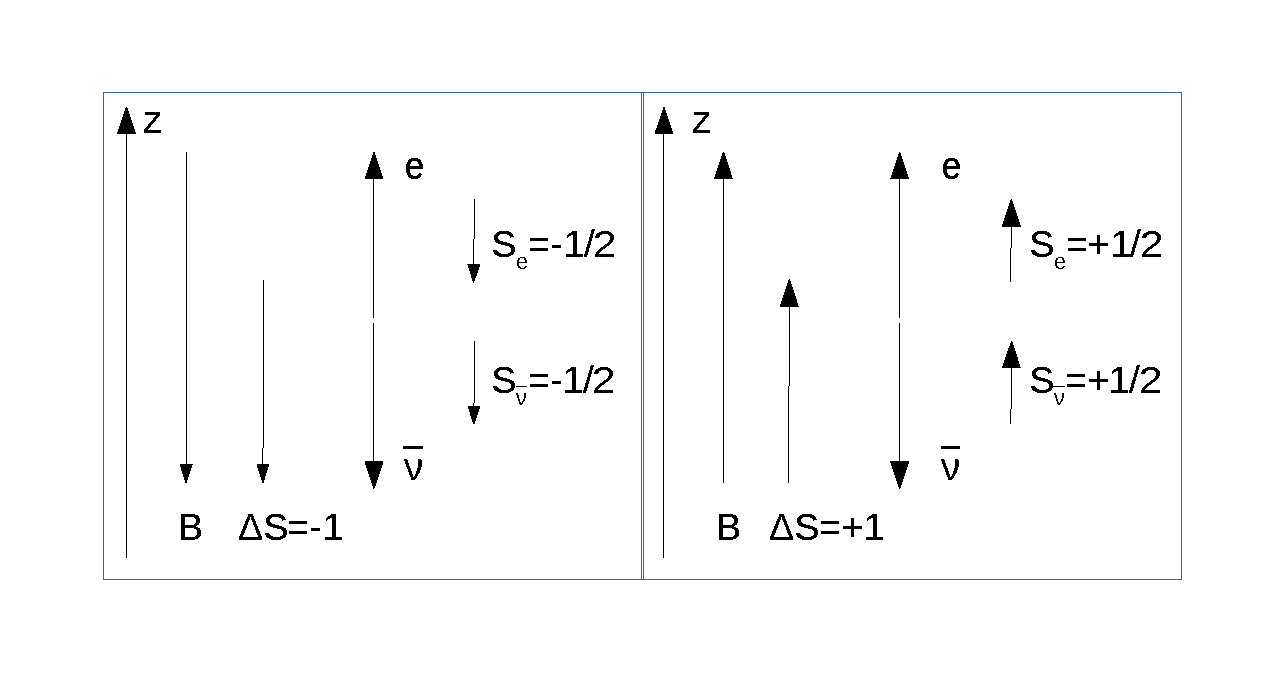
\includegraphics[width=0.6\linewidth]{DibujoExamen.pdf}
\end{center}
\caption{Visión esquemática del experimento de Madame Wu para dos configuraciones opuestas de campo magnético.}
\label{dibujo}
\end{figure}






\end{document}
